\documentclass{standalone}
\usepackage{tikz}
\usetikzlibrary{patterns, positioning}
\usepackage[sfdefault]{ClearSans} %% option 'sfdefault' activates Clear Sans as the default text font
\usepackage[T1]{fontenc}

\begin{document}
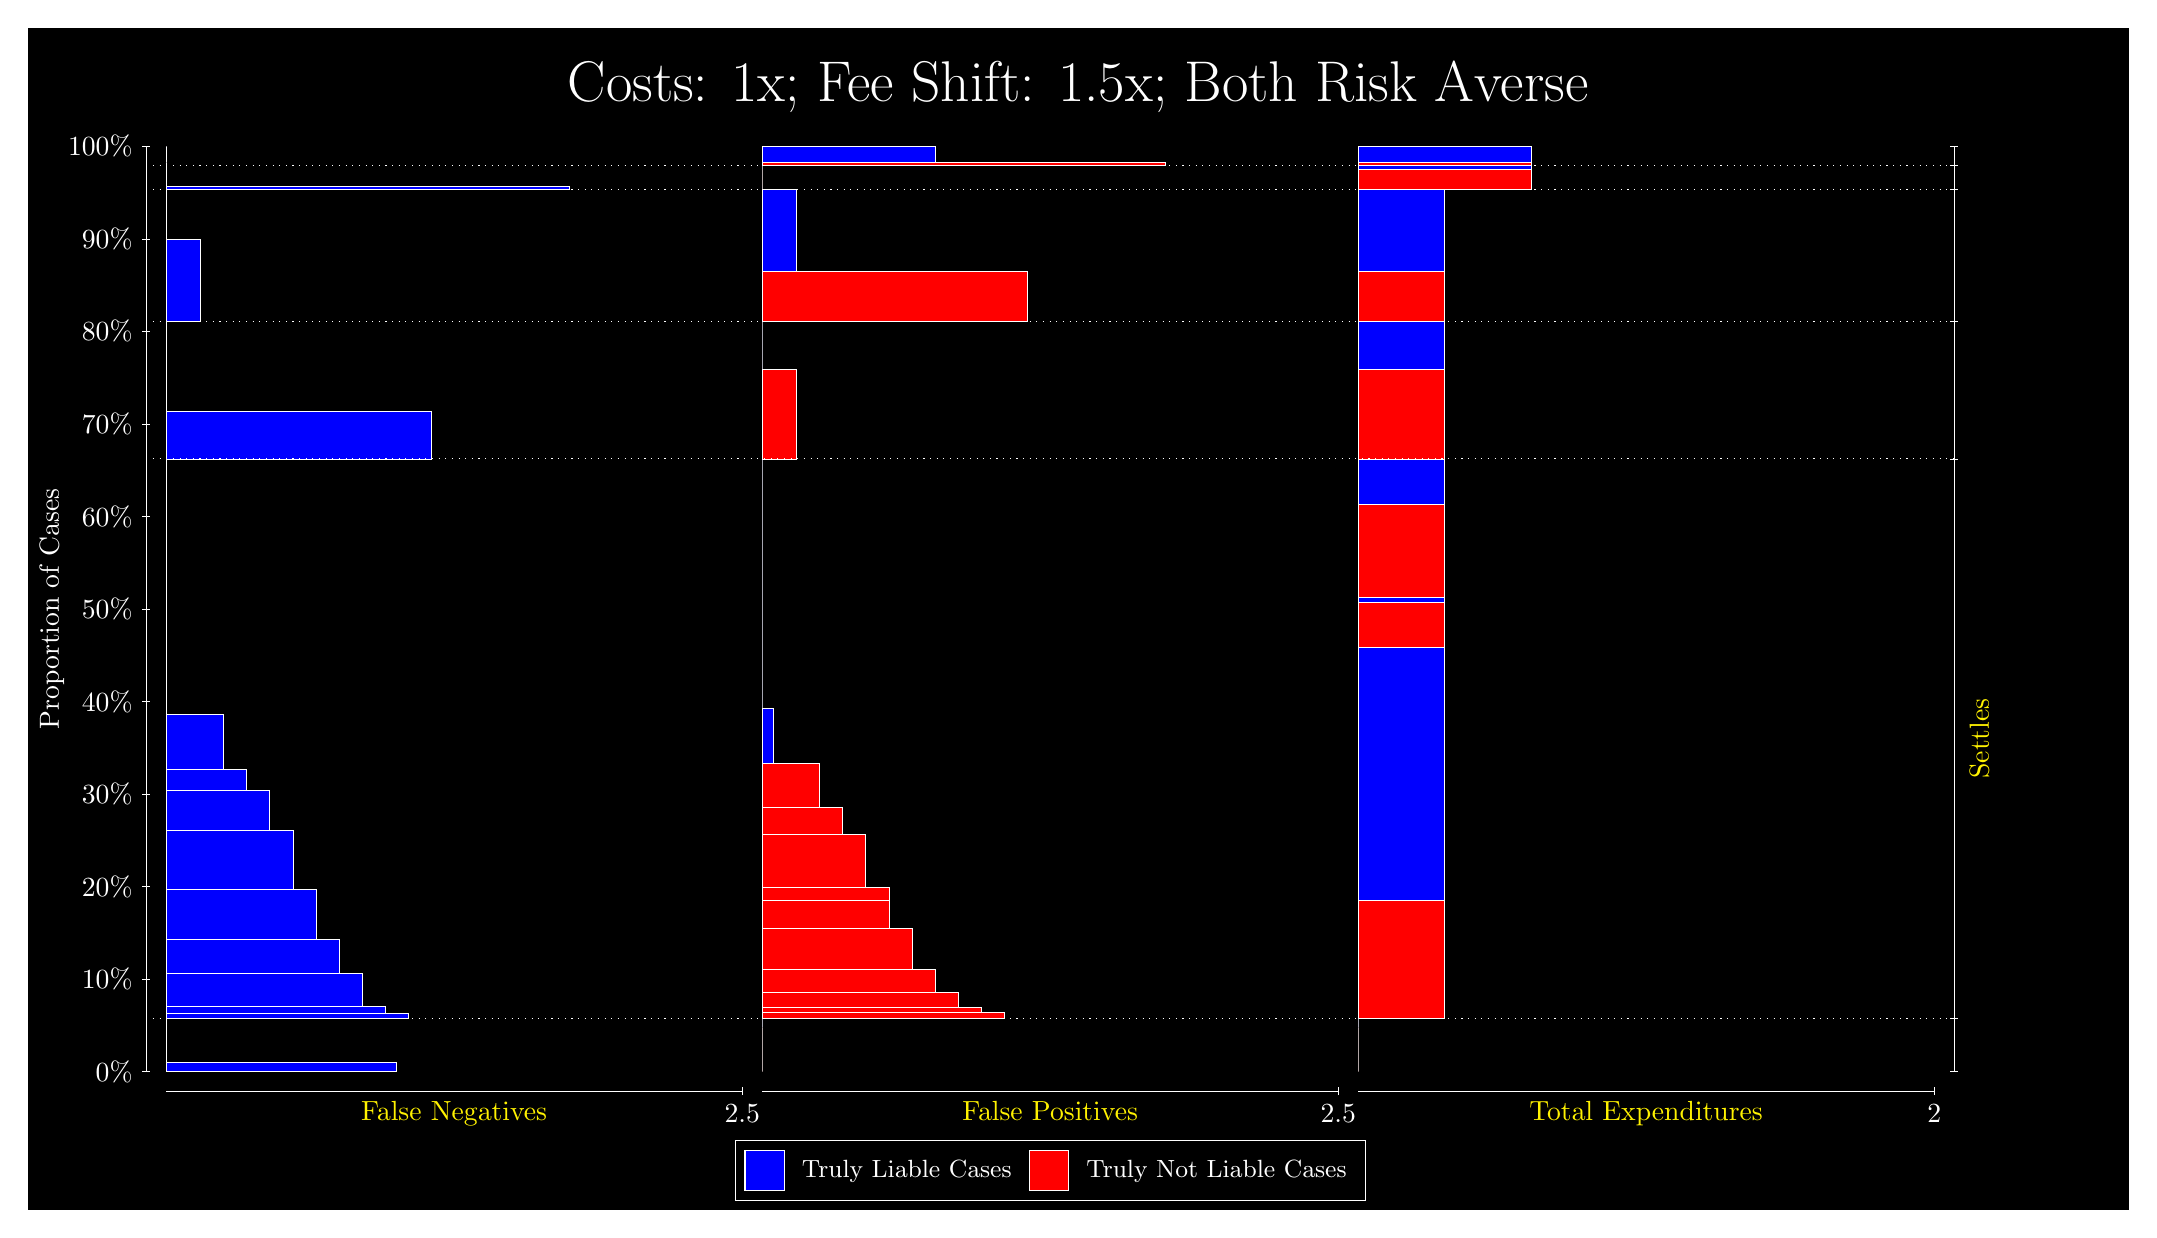
\begin{tikzpicture}
\draw[fill=black] (0,0) rectangle (26.667,15);
\draw[text=white] (0,13.5) rectangle (26.667,15) node[midway] {\huge Costs: 1x; Fee Shift: 1.5x; Both Risk Averse};
\draw[white, very thin] (1.5,1.75) -- (1.5,13.5);
\node[rotate=90, text=white, anchor=center] at (0.3, 7.625) {Proportion of Cases};
\draw[white, very thin] (1.45,1.75) -- (1.55,1.75);
\node[text=white, anchor=east] at (1.45, 1.75) {0\%};
\draw[white, very thin] (1.45,2.925) -- (1.55,2.925);
\node[text=white, anchor=east] at (1.45, 2.925) {10\%};
\draw[white, very thin] (1.45,4.1) -- (1.55,4.1);
\node[text=white, anchor=east] at (1.45, 4.1) {20\%};
\draw[white, very thin] (1.45,5.275) -- (1.55,5.275);
\node[text=white, anchor=east] at (1.45, 5.275) {30\%};
\draw[white, very thin] (1.45,6.45) -- (1.55,6.45);
\node[text=white, anchor=east] at (1.45, 6.45) {40\%};
\draw[white, very thin] (1.45,7.625) -- (1.55,7.625);
\node[text=white, anchor=east] at (1.45, 7.625) {50\%};
\draw[white, very thin] (1.45,8.8) -- (1.55,8.8);
\node[text=white, anchor=east] at (1.45, 8.8) {60\%};
\draw[white, very thin] (1.45,9.975) -- (1.55,9.975);
\node[text=white, anchor=east] at (1.45, 9.975) {70\%};
\draw[white, very thin] (1.45,11.15) -- (1.55,11.15);
\node[text=white, anchor=east] at (1.45, 11.15) {80\%};
\draw[white, very thin] (1.45,12.325) -- (1.55,12.325);
\node[text=white, anchor=east] at (1.45, 12.325) {90\%};
\draw[white, very thin] (1.45,13.5) -- (1.55,13.5);
\node[text=white, anchor=east] at (1.45, 13.5) {100\%};

\draw[white, very thin] (24.457,1.75) -- (24.457,13.5);
\draw[white, very thin] (24.407,1.75) -- (24.507,1.75);
\node[anchor=west] at (24.407, 1.75) {};
\draw[white, very thin] (24.407,2.426) -- (24.507,2.426);
\node[anchor=west] at (24.407, 2.426) {};
\draw[white, very thin] (24.407,9.5317) -- (24.507,9.5317);
\node[anchor=west] at (24.407, 9.5317) {};
\draw[white, very thin] (24.407,11.274) -- (24.507,11.274);
\node[anchor=west] at (24.407, 11.274) {};
\draw[white, very thin] (24.407,12.955) -- (24.507,12.955);
\node[anchor=west] at (24.407, 12.955) {};
\draw[white, very thin] (24.407,13.254) -- (24.507,13.254);
\node[anchor=west] at (24.407, 13.254) {};
\draw[white, very thin] (24.407,13.5) -- (24.507,13.5);
\node[anchor=west] at (24.407, 13.5) {};

\draw[white, very thin, fill=blue] (1.75,1.75) rectangle (4.6775,1.8664);
\draw[white, very thin, fill=red] (1.75,1.8664) rectangle (1.75,2.426);
\draw[white, very thin, fill=blue] (1.75,2.426) rectangle (4.8239,2.4904);
\draw[white, very thin, fill=blue] (1.75,2.4904) rectangle (4.5312,2.5807);
\draw[white, very thin, fill=blue] (1.75,2.5807) rectangle (4.2384,3.0034);
\draw[white, very thin, fill=blue] (1.75,3.0034) rectangle (3.9457,3.4267);
\draw[white, very thin, fill=blue] (1.75,3.4267) rectangle (3.6529,4.0623);
\draw[white, very thin, fill=blue] (1.75,4.0623) rectangle (3.3602,4.8122);
\draw[white, very thin, fill=blue] (1.75,4.8122) rectangle (3.0674,5.3201);
\draw[white, very thin, fill=blue] (1.75,5.3201) rectangle (2.7746,5.5897);
\draw[white, very thin, fill=blue] (1.75,5.5897) rectangle (2.4819,6.2919);
\draw[white, very thin, fill=red] (1.75,6.2919) rectangle (1.75,9.5317);
\draw[white, very thin, fill=blue] (1.75,9.5317) rectangle (5.1167,10.136);
\draw[white, very thin, fill=red] (1.75,10.136) rectangle (1.75,11.274);
\draw[white, very thin, fill=blue] (1.75,11.274) rectangle (2.1891,12.317);
\draw[white, very thin, fill=red] (1.75,12.317) rectangle (1.75,12.955);
\draw[white, very thin, fill=blue] (1.75,12.955) rectangle (6.8732,12.997);
\draw[white, very thin, fill=red] (1.75,12.997) rectangle (1.75,13.254);
\draw[white, very thin, fill=red] (1.75,13.254) rectangle (1.75,13.297);
\draw[white, very thin, fill=blue] (1.75,13.297) rectangle (1.75,13.5);
\draw[white, very thin, fill=red] (9.3189,1.75) rectangle (9.3189,2.3097);
\draw[white, very thin, fill=blue] (9.3189,2.3097) rectangle (9.3189,2.426);
\draw[white, very thin, fill=red] (9.3189,2.426) rectangle (12.393,2.504);
\draw[white, very thin, fill=red] (9.3189,2.504) rectangle (12.1,2.568);
\draw[white, very thin, fill=red] (9.3189,2.568) rectangle (11.807,2.7584);
\draw[white, very thin, fill=red] (9.3189,2.7584) rectangle (11.515,3.048);
\draw[white, very thin, fill=red] (9.3189,3.048) rectangle (11.222,3.5683);
\draw[white, very thin, fill=red] (9.3189,3.5683) rectangle (10.929,3.9224);
\draw[white, very thin, fill=red] (9.3189,3.9224) rectangle (10.929,4.0906);
\draw[white, very thin, fill=red] (9.3189,4.0906) rectangle (10.636,4.7668);
\draw[white, very thin, fill=red] (9.3189,4.7668) rectangle (10.344,5.1001);
\draw[white, very thin, fill=red] (9.3189,5.1001) rectangle (10.051,5.6658);
\draw[white, very thin, fill=blue] (9.3189,5.6658) rectangle (9.4652,6.3681);
\draw[white, very thin, fill=blue] (9.3189,6.3681) rectangle (9.3189,9.5317);
\draw[white, very thin, fill=red] (9.3189,9.5317) rectangle (9.758,10.67);
\draw[white, very thin, fill=blue] (9.3189,10.67) rectangle (9.3189,11.274);
\draw[white, very thin, fill=red] (9.3189,11.274) rectangle (12.686,11.912);
\draw[white, very thin, fill=blue] (9.3189,11.912) rectangle (9.758,12.955);
\draw[white, very thin, fill=red] (9.3189,12.955) rectangle (9.3189,13.212);
\draw[white, very thin, fill=blue] (9.3189,13.212) rectangle (9.3189,13.254);
\draw[white, very thin, fill=red] (9.3189,13.254) rectangle (14.442,13.297);
\draw[white, very thin, fill=blue] (9.3189,13.297) rectangle (11.515,13.5);
\draw[white, very thin, fill=red] (16.888,1.75) rectangle (16.888,2.3097);
\draw[white, very thin, fill=blue] (16.888,2.3097) rectangle (16.888,2.426);
\draw[white, very thin, fill=red] (16.888,2.426) rectangle (17.986,3.9224);
\draw[white, very thin, fill=blue] (16.888,3.9224) rectangle (17.986,7.1436);
\draw[white, very thin, fill=red] (16.888,7.1436) rectangle (17.986,7.7093);
\draw[white, very thin, fill=blue] (16.888,7.7093) rectangle (17.986,7.7737);
\draw[white, very thin, fill=red] (16.888,7.7737) rectangle (17.986,8.9513);
\draw[white, very thin, fill=blue] (16.888,8.9513) rectangle (17.986,9.5317);
\draw[white, very thin, fill=red] (16.888,9.5317) rectangle (17.986,10.67);
\draw[white, very thin, fill=blue] (16.888,10.67) rectangle (17.986,11.274);
\draw[white, very thin, fill=red] (16.888,11.274) rectangle (17.986,11.912);
\draw[white, very thin, fill=blue] (16.888,11.912) rectangle (17.986,12.955);
\draw[white, very thin, fill=red] (16.888,12.955) rectangle (19.083,13.212);
\draw[white, very thin, fill=blue] (16.888,13.212) rectangle (19.083,13.254);
\draw[white, very thin, fill=red] (16.888,13.254) rectangle (19.083,13.297);
\draw[white, very thin, fill=blue] (16.888,13.297) rectangle (19.083,13.5);
\draw[white, dotted] (1.5,2.426) -- (24.457,2.426);
\draw[white, dotted] (1.5,9.5317) -- (24.457,9.5317);
\draw[white, dotted] (1.5,11.274) -- (24.457,11.274);
\draw[white, dotted] (1.5,12.955) -- (24.457,12.955);
\draw[white, dotted] (1.5,13.254) -- (24.457,13.254);
\draw[white, very thin] (1.75,1.5) -- (9.0689,1.5);
\node[text=yellow, anchor=north] at (5.4094, 1.5) {False Negatives};
\draw[white, very thin] (9.0689,1.45) -- (9.0689,1.55);
\node[text=white, anchor=north] at (9.0689, 1.45) {2.5};

\draw[white, very thin] (9.3189,1.5) -- (16.638,1.5);
\node[text=yellow, anchor=north] at (12.978, 1.5) {False Positives};
\draw[white, very thin] (16.638,1.45) -- (16.638,1.55);
\node[text=white, anchor=north] at (16.638, 1.45) {2.5};

\draw[white, very thin] (16.888,1.5) -- (24.207,1.5);
\node[text=yellow, anchor=north] at (20.547, 1.5) {Total Expenditures};
\draw[white, very thin] (24.207,1.45) -- (24.207,1.55);
\node[text=white, anchor=north] at (24.207, 1.45) {2};


\node[text=yellow, centered, rotate=90] at (24.777, 5.9789) {Settles};





\draw (12.978300999999998,1.5) node[draw=none] (baseCoordinate) {};
\begin{scope}[align=center]
        \matrix[scale=0.5, draw=white, below=0.5cm of baseCoordinate, nodes={draw}, column sep=0.1cm]{
            \node[rectangle, draw, minimum width=0.5cm, minimum height=0.5cm, fill=blue] {}; &
            \node[draw=none, font=\small, text=white] (B) {Truly Liable Cases}; &
            \node[rectangle, draw, minimum width=0.5cm, minimum height=0.5cm, fill=red] {}; &
            \node[draw=none, font=\small, text=white] (B) {Truly Not Liable Cases}; \\
            };
\end{scope}

\end{tikzpicture}
\end{document}